\documentclass[10pt,a4paper]{article}
\usepackage[margin=20mm]{geometry}
\usepackage[T1]{fontenc}\usepackage[utf8]{inputenc}
\usepackage{lmodern,microtype,amsmath,amssymb,booktabs,tabularx,longtable,graphicx,caption,xcolor,titlesec,fancyhdr,hyperref,xurl}
\setcounter{secnumdepth}{-1}
\definecolor{ink}{HTML}{17252A}\definecolor{teal}{HTML}{176B68}\definecolor{gold}{HTML}{B8892F}
\hypersetup{colorlinks=true,linkcolor=teal,urlcolor=teal,citecolor=teal,pdftitle={Available Evidence Is Not Engineering Authority},pdfauthor={Joseph Maxwell}}
\titleformat{\section}{\Large\bfseries\sffamily\color{ink}}{\thesection}{0.6em}{}\titleformat{\subsection}{\large\bfseries\sffamily\color{teal}}{\thesubsection}{0.6em}{}
\captionsetup{font=small,labelfont=bf,justification=raggedright,singlelinecheck=false}
\pagestyle{fancy}\fancyhf{}\fancyhead[L]{\small\sffamily MATERIALS ML FAILURE ANALYSIS}\fancyhead[R]{\small\sffamily FINAL QA V3}\fancyfoot[C]{\small\thepage}\setlength{\headheight}{15pt}
\setlength{\parindent}{0pt}\setlength{\parskip}{5pt plus 1pt}\setlength{\emergencystretch}{2em}
\newcommand{\plainbox}[1]{\begin{center}\fcolorbox{teal}{teal!5}{\begin{minipage}{0.92\linewidth}#1\end{minipage}}\end{center}}
\title{Available Evidence Is Not Engineering Authority\\\large Admission, viability, replay, and bounded action in computational engineering}
\author{Joseph Maxwell\\\small The Systemica Institute, London, United Kingdom\\\small ORCID: \href{https://orcid.org/0009-0002-4070-6035}{0009-0002-4070-6035}\\\small \href{mailto:j.maxwell@systemicainstitute.org}{j.maxwell@systemicainstitute.org}}
\date{Preprint -- August 2026}
\begin{document}\maketitle

\begin{abstract}
Computational evidence can support a weak claim without supporting the stronger action that follows it. This paper synthesises previously generated frozen evidence from materials-informatics and bounded engineering studies; no new scientific model fitting was performed for the synthesis itself. A prospective no-fit review of 26,056 Materials Project elastic record-target pairs found 23,891 conditionally usable and 2,165 anomalous or unresolved under a predeclared rubric. Among the same 288 elastic model-evaluation cells, 73.3\% beat paired target-permutation nulls but only 4.51\% achieved positive held-out $R^2$. Repeated executions also reached different outcomes: Matbench and the final spatial route repeated exactly at their declared scientific levels, whereas Materials Project elasticity retained 916 numerical exceedances. Three bounded engineering studies then showed why these distinctions matter at an action boundary. Together the witnesses show that source suitability, predictive viability, reproducibility, and engineering permission are different questions. The paper does not establish universal admission rules, external replication, physical qualification, regulatory compliance, retrospective full-stack validation, or universal cross-domain validity.
\end{abstract}

\plainbox{\textbf{This paper in plain language}\par
\textbf{Question:} When does a computational result earn permission to influence an engineering decision?\par
\textbf{Why it matters:} More computation does not automatically create a stronger or safer decision.\par
\textbf{What we did:} We traced source suitability, prediction, repeat/replay, and bounded action through materials-ML experiments and three engineering studies.\par
\textbf{What we found:} A result can exist without being suitable, contain signal without being viable, replay exactly while preserving a failure, or be scientifically accepted without authorising fabrication.\par
\textbf{What it does not mean:} The sequence is a locally demonstrated decision framework, not a universal law of engineering.}

\noindent\textbf{Three ways to read this paper.} \textbf{Just want the answer?} Read the box, the five-state chain below, and the Conclusion. \textbf{Want the evidence?} Read Sections 3--7. \textbf{Want to audit it?} Follow the public receipts, scale register, claim boundaries, and reconstruction package.

\begin{center}\small
\begin{tabularx}{0.98\linewidth}{@{}>{\centering\arraybackslash}X>{\centering\arraybackslash}X>{\centering\arraybackslash}X>{\centering\arraybackslash}X>{\centering\arraybackslash}X@{}}
\textbf{AVAILABLE} & \textbf{ADMITTED} & \textbf{VIABLE} & \textbf{REPLAYED} & \textbf{ACTION-BOUNDED}\\
Do I have a value? & Can I use it for this purpose? & Does the model clear the declared test? & What happened when it ran again? & What may happen next?\\
\end{tabularx}
\end{center}

\section{1. Introduction: From a result to a decision}
A value can exist without being suitable for a strong scientific claim. A suitable source can still produce a poor model. A useful model can still fail to reproduce. A reproducible result can still be insufficient to justify an engineering action.

These distinctions matter because computational outputs affect what happens next. A database value may enter a training cohort. A model may advance a material to higher-fidelity calculation. A repeated result may be treated as validated. An attractive simulation may trigger fabrication. At each step, a weaker result can silently acquire the practical force of a stronger one.

The central proposition is therefore simple:
\begin{quote}\textbf{A weaker evidence object should not silently inherit the authority of a stronger one.}\end{quote}
Here, authority means only the decision that a result is strong enough to justify. It does not mean that one framework replaces scientific judgement.

We test the proposition using four kinds of empirical witness: a Materials Project source review, a Materials Project predictive failure, five measured repeat/replay routes, and three bounded engineering case studies. The compact chain introduced after those plain distinctions is
\[
\mathrm{AVAILABLE}\rightarrow\mathrm{ADMITTED}\rightarrow\mathrm{VIABLE}
\rightarrow\mathrm{REPLAY\!\mbox{-}ADJUDICATED}\rightarrow\mathrm{ACTION\!\mbox{-}BOUNDED}.
\]
``Admitted'' means suitable for the declared scientific use. ``Viable'' means meeting the declared absolute predictive baseline. ``Replay-adjudicated'' means a new execution identity was compared under an explicit contract. ``Action-bounded'' means the evidence supports only a specified next step.

The sequence is a decision-ordering device for this programme, not a claim that every computational workflow has identical states or must traverse them linearly.

The empirical validation is materials-specific. Execution, comparison, memory, and decision-boundary logic may be portable, but cross-domain scientific usefulness remains a transfer hypothesis.

\section{2. How the proposition was tested}
Table~\ref{tab:witnesses} gives the reader map. Each witness tests a different substitution. No witness is used to upgrade another.

\begin{table}[htbp]\centering\small
\caption{Empirical witnesses and the questions they test.}\label{tab:witnesses}
\begin{tabularx}{\linewidth}{@{}p{0.20\linewidth}p{0.21\linewidth}p{0.24\linewidth}X@{}}\toprule
Witness & Object tested & Public protocol & Question\\\midrule
Materials Project admission & 26,056 elastic record-target pairs & Frozen no-fit source review & Is an available value sufficiently specified for the stronger scientific claim?\\
Materials Project viability & 288 paired-null-comparable model cells & Null separation plus absolute $R^2$ & Does target-linked signal also cross the declared positive-$R^2$ boundary?\\
JARVIS, MP, Matbench, Spatial & Fresh and replay outputs & Declared comparison contracts & What exactly repeated: workload, meaning, numbers, or bytes?\\
Engineering cases & Three bounded design studies & Explicit human stop/next-test boundary & What action, if any, did the computation justify?\\\bottomrule
\end{tabularx}\end{table}

The materials audits used frozen datasets, cohorts, models, controls, and comparison rules. The engineering studies used deterministic local solvers and explicit limitations. No new scientific fit was performed for this synthesis.

\section{3. Available is not admitted}
\subsection{3.1 Plain comparison}
Property presence answers: \emph{is a value available?} A stronger scientific use asks: \emph{are its units, convention, method, and physical meaning adequate for this claim?} We call the second check source admission.

For elasticity, a scalar modulus can depend on tensor consistency, averaging convention, calculation method, and mechanical stability. A negative or extreme value is not automatically corrupt. It may be physically meaningful, unstable, convention-dependent, or erroneous. Magnitude therefore begins an investigation; it does not finish one.

\subsection{3.2 Measured result}
A prospective no-fit audit classified 26,056 Materials Project elastic record-target pairs. It retained 23,891 as conditional and 2,165 as anomalous or unresolved. Zero reached the strongest category under the predeclared admission rubric used in this study because the available scalar summaries lacked the tensor- and method-level evidence required by that category (Figure~\ref{fig:admission}).

\begin{figure}[htbp]\centering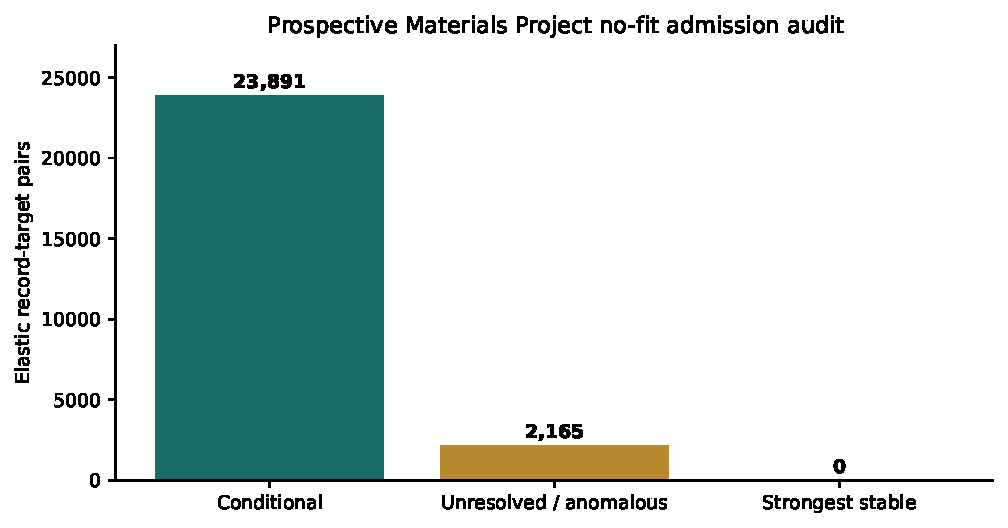
\includegraphics[width=0.80\linewidth]{figures/PAPER_3_MP_ADMISSION.pdf}\caption{\textbf{Having a source value did not automatically make it suitable for the strongest declared use.} The no-fit review retained conditional and unresolved records instead of silently deleting them.}\label{fig:admission}\end{figure}

The result does not say that every record is wrong or that the Materials Project is unusable. It says that the strongest elastic claim required evidence that the scalar route did not contain. The practical outcome was a request for tensor-bearing records, record-level method evidence, expert review, and prospectively frozen memberships.

\section{4. Admitted is not viable}
An admitted target may still be poorly represented by a model. Conversely, a statistically promising model may still rest on unresolved source semantics. These are independent questions.

The Materials Project model audit supplied a direct contradiction. For each eligible valid cell, the paired null was the mean $R^2$ from 30 otherwise matched models trained on permuted targets. Of the same 288 elastic cells, 211 (73.3\%) beat that broken-target comparator. Only 13 (4.51\%) achieved $R^2>0$, and the same 13 passed both tests. All 13 were bulk-modulus cells. Across the wider 1,152-cell elastic route, only 20 (1.74\%) had positive $R^2$ and median $R^2$ was $-2.248$.

The first test asks whether the valid route learned target-linked signal. The second asks whether it reduced squared error relative to predicting the mean of the evaluated targets. Beating the broken comparator did not imply even this minimal absolute performance. The $R^2>0$ boundary is not a universal engineering threshold; most applications require more.

\section{5. Completed is not replayed}
\subsection{5.1 Fresh, resume, and replay}
A fresh execution starts a new scientific identity. Resume continues the same interrupted identity after verifying completed units and rerunning incomplete ones. Replay starts a new identity with an explicit predecessor and independently executes the complete frozen plan. Resume tests controlled continuation; replay tests repeatability.

A repeat is a separately identified execution of the same scientific experiment under the declared environment. External replication requires an independent group, environment, or implementation and was not achieved here. Resume is not replication, and replay is not automatically external replication.

\textbf{Scientific unit:} one complete, independently committable part of the declared experiment. It binds the source, task, split or fold, model or representation, seed or condition, required outputs, and execution identity. It commits only after those outputs and identities validate. A unit is not a fixed amount of computation: it may contain one fit, several fits, a control set, or a solver calculation. For example, \textbf{20 Matbench V0.2 scientific units represented 120 estimator fits}.

A replay contract must also say what is compared. The ordered plan may match while raw files differ. Numeric values may match while timestamps do not. Byte identity may coexist with a scientifically mixed conclusion. ``Reproduced'' is therefore incomplete unless the matching contract is stated.

\subsection{5.2 Measured replay states}
\begin{table}[htbp]\centering\scriptsize
\caption{The programme retained different repeat/replay outcomes rather than forcing one PASS label.}
\begin{tabularx}{\linewidth}{@{}p{0.18\linewidth}p{0.25\linewidth}X@{}}\toprule
Route & Comparison scope & Observed result\\\midrule
JARVIS & 48 fresh + 48 replay; 28,248 numeric cells & Maximum difference about $1.07\times10^{-14}$; numerical equivalence; 60/192 files byte-divergent\\
Materials Project & 64 fresh + 64 replay; 37,924 numeric cells & 916 strict exceedances, all elastic; adverse divergence retained\\
Matbench & 3,440 fresh + 3,440 repeat; 65,740 numeric cells & Zero numeric differences; semantic identity PASS\\
Spatial V0.5 & 256 fresh + 256 replay & Byte, semantic, and numeric identity PASS\\
Spatial V0.6.1 & 576 fresh + 576 replay; 1,728 output pairs; 927,361 cells & Exact byte, semantic, and numeric replay; bulk geometry passed both views; shear polarity remained conditional\\\bottomrule
\end{tabularx}\end{table}

\begin{figure}[htbp]\centering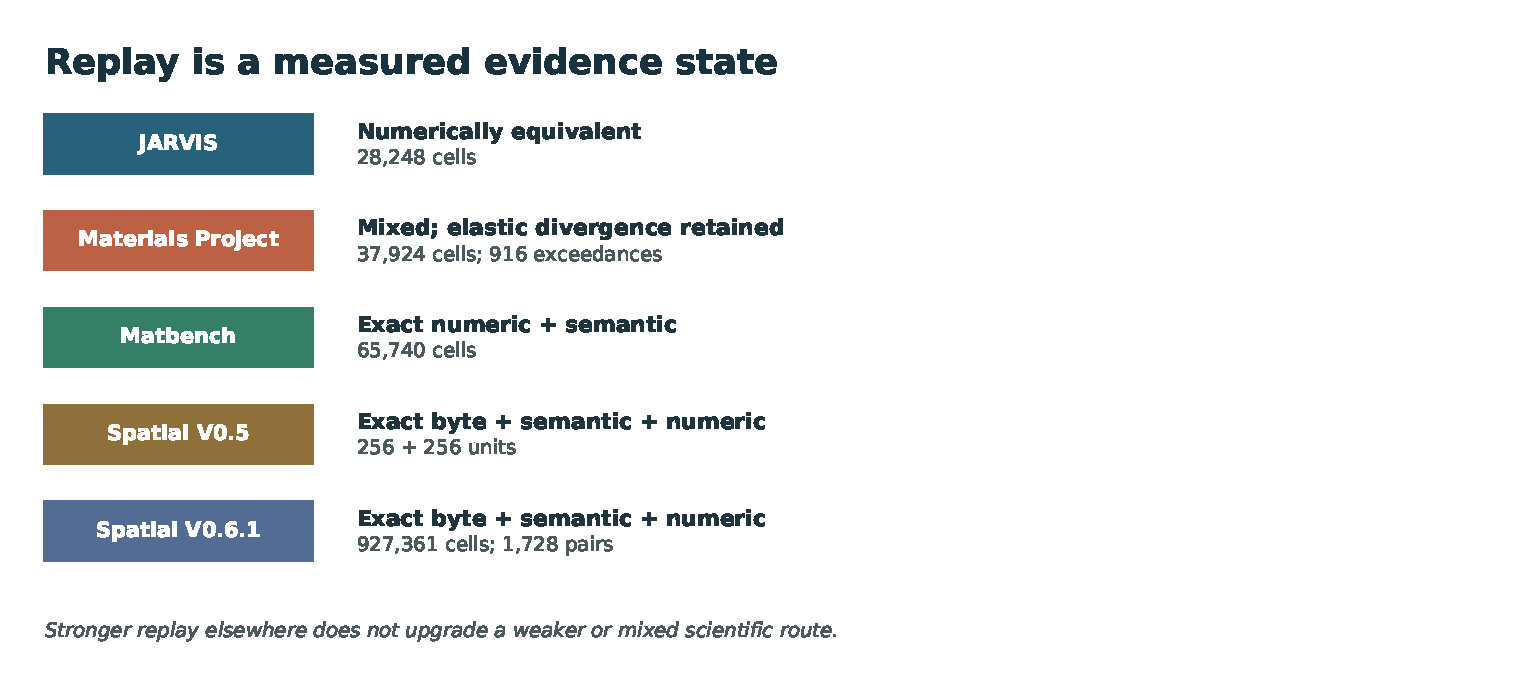
\includegraphics[width=0.91\linewidth]{figures/PAPER_3_REPLAY_STATES.pdf}\caption{\textbf{Running work again did not force every route into one PASS state.} Different workloads reached different declared repeat/replay outcomes, and counts retain their own denominators.}\end{figure}

The central lesson is plain: \textbf{repeating a computation does not automatically strengthen the scientific claim; it can reproduce a failure or a conditional result exactly.} Spatial V0.6.1 is the clearest example. Its exact replay preserved both the bulk PASS and the shear cross-view failure.

\section{6. Beyond Materials ML: Three Bounded Engineering Witnesses}
\subsection{6.1 Why the problem stopped being only a materials-ML problem}
Materials ML first exposed evidence substitutions in a controlled scientific setting: fitted importance could diverge from retrained consequence; null separation could coexist with negative absolute performance; and repeatability could coexist with a held scientific result. The engineering studies then showed analogous failures at the action boundary. A thermal result stopped transferring after geometry changed. A tank route could be computationally evaluable while containing invalid state transitions. A heat-shield design could improve containment while degrading thermal performance. The shared problem was therefore not a particular materials model. It was the transition from computational result to justified next action.

\begin{center}\small\bfseries
MATERIALS ML: What does the model or evidence actually support?\\[2pt]
$\downarrow$ repeated failure modes become visible $\downarrow$\\[2pt]
GENERAL COMPUTATIONAL ENGINEERING: What may the result legitimately change next?
\end{center}

The engineering cases show transferable control behaviour across three local computational engineering studies. They do not constitute retrospective validation of the complete modern Systemica architecture, physical validation, external validation, or industrial deployment.

\begin{table}[htbp]\centering\scriptsize
\caption{Local engineering witnesses and their bounded outcomes.}
\begin{tabularx}{\linewidth}{@{}p{0.12\linewidth}p{0.17\linewidth}p{0.25\linewidth}p{0.20\linewidth}X@{}}\toprule
Case & Engineering problem & Failure or contradiction exposed & Control behaviour exercised & Bounded next action\\\midrule
Furnace & Thermal-interface design & Correcting 350--375 mm to 35--40 mm broke transfer of an inherited 59.2~$^\circ$C result; active cooling introduced a failure dependency & Case identity, uncertainty/fault scenarios, predecessor-transfer refusal & Guarded opaque thermal-interface coupon; no fabrication or furnace operation\\
Dual tank & State, provenance, topology & Fresh reserve, live feeder/recovery, and returned/consumed states could not be collapsed; forbidden return routes were rejected & Typed state/topology and transition validation & Low-pressure non-potable tracer rig; no deployment\\
Heat shield & Thermal-flow and fault containment & Segmentation improved containment while degrading thermal performance; adverse cases were retained & Competing-objective and failure-case retention & Matched cold-flow/heated coupons with blocked-cell and contained-leak cases; no qualification\\
\bottomrule\end{tabularx}\end{table}

Across the three cases, 13 candidate objects, five descendants, 116 scenario runs, 9,150 parameter or uncertainty runs, and at least 9,380 model operations narrowed broad concepts to smaller falsifiable tests. These counts do not measure cost savings or provide physical validation.

The furnace object was a high-temperature brazing-furnace enclosure and removable optical/thermal viewport interface. Its bounded model used dominant-path thermal-resistance screening, candidate-specific heat paths, six open/fault scenarios, and 9,000 deterministic uncertainty samples (9,120 model operations). It varied geometry, aperture, emissivity, hot-side boundary, contact and seal assumptions, cooling loss, and unresolved edge/frame transfer. The calculation showed why the inherited temperature no longer belonged to the corrected geometry and why active cooling introduced a new dependency.

The dual-tank object was a reserve/feeder/recovery water topology. A lumped flow/state model and typed transition checks separated new-source reserve, live feeder/recovery, unused return, consumed water, and contained/rejected states. Twenty-six scenarios and 70 parameter cases rejected forbidden return routes before execution. The strongest descendant improved an exploratory worst service margin from $-0.266$ to $-0.090$ but did not resolve sizing, hygiene, pressure loss, or water quality.

The heat-shield object was a segmented porous/transpiration ground-coupon concept. Its model coupled a two-node-per-cell transient thermal network with Darcy-style restricted flow and topology/fault checks across 84 scenarios and 80 parameter cases. The monolithic control produced the stronger nominal thermal range (175.3--389.5 K reduction), while the segmented route included outcomes from $-83.5$ to 245.4 K and better localised blockage/leak information. Pore-scale convection, compressibility, film formation, oxidation, erosion, contacts, and flight aerothermodynamics remained unresolved.

The technical contribution is the design synthesis and engineering reduction demonstrated within the programme, not a claim of literature-level novelty for every physical mechanism.

\subsection{6.2 Architecture lineage, not retrospective architecture}
Repeated behaviours observed across case-specific scientific and engineering workflows were progressively formalised into reusable execution, evidence, replay, memory, state, and bounded-authority services. The later architecture was not retrospectively present in full in the historical cases.

\begin{table}[htbp]\centering\small
\caption{Recurring needs and their later reusable expression.}
\begin{tabularx}{\linewidth}{@{}X X@{}}\toprule
Recurrent case-study need & Later reusable architectural expression\\\midrule
What exactly is the case or state? & Typed source, mission, and state identity\\
Which transitions are invalid? & State, topology, and transition validation\\
What happens under perturbation or failure? & Governed stress and failure evidence\\
What survives interruption? & Recovery and checkpoint verification\\
What repeats under a separately identified replay? & Replay contracts\\
Can this progress to fabrication or deployment? & Bounded authority and HOLD\\
\bottomrule\end{tabularx}\end{table}

This mapping is architectural lineage, not evidence that the later modules were already present in full in the historical runs.

Scientific-domain transfer is not established outside the demonstrated materials semantics. Control-logic transfer has initial local evidence across materials ML/data analysis, thermal-interface design, fluid/state topology, and thermal-flow/fault-containment design. The case studies provide initial local evidence that explicit identity, state validity, failure retention, replay, and bounded next-action logic remain useful across several computational engineering problem types. They do not establish universal cross-domain validity.

\section{7. Execution and memory implications}
\subsection{7.1 If a long computation stops, what can be trusted?}
Scientific work was divided into declared units with expected outputs. A unit counted as complete only after its outputs passed validation. On resume, verified units were retained and incomplete units rerun. This makes interruption recovery inspectable without turning resume into replay.

\begin{center}\small\bfseries
DECLARED UNIT $\rightarrow$ LOCAL STAGING $\rightarrow$ FILE/SCHEMA/IDENTITY CHECKS $\rightarrow$ ATOMIC COMMIT $\rightarrow$ JOURNAL/CHECKPOINT
\end{center}
Only complete contract-valid units advanced accepted execution state. A visible partial file was not treated as completion. The operating rule was: \textbf{resume from the last verified scientific boundary, not from the last visible file.}

This was exercised rather than merely proposed. The JARVIS replay was interrupted and resumed under the same identity; incomplete staging was rejected and recomputed. The Materials Project replay also used a later resume launch while retaining only verified complete units. A separate controlled-fixture campaign terminated child processes at 11 declared fault boundaries and recovered each fixture to three unique committed units. Those 11 terminations are controller evidence, not 11 scientific experiments.

\begin{table}[htbp]\centering\scriptsize
\caption{Publicly evidenced programme scale. Unlike objects remain separate.}
\begin{tabularx}{\linewidth}{@{}p{0.18\linewidth}r r r X@{}}\toprule
Route & Fresh & Repeat/replay & Unit executions & Additional evidence\\\midrule
JARVIS & 48 & 48 & 96 & 28,248 numeric cells; 192 file pairs\\
Materials Project & 64 & 64 & 128 & 37,924 cells; 916 elastic exceedances\\
Matbench V0.2 & 20 & 0 & 20 & 120 estimator fits\\
Matbench V0.3 & 3,440 & 3,440 & 6,880 & 6,880 fits; 65,740 compared cells\\
Spatial V0.5 & 256 & 256 & 512 & byte, semantic, numeric PASS\\
Spatial V0.6.1 & 576 & 576 & 1,152 & 1,728 output pairs; 927,361 cells\\
Other sealed spatial predecessors & 28 & 20 & 48 & V0.1--V0.4, classified separately\\\midrule
Total committed units & 4,432 & 4,404 & 8,836 & Not a fit or operation total\\\bottomrule
\end{tabularx}\end{table}

At least 1,059,273 explicitly counted numeric fresh-to-repeat/replay comparison cells were adjudicated across routes exposing cell-level counts. This is not the total number of calculations performed. The principal workstation was shared rather than dedicated. Calendar duration therefore includes ordinary use, review, interruption, and unmeasured gaps; it is not runtime. The scientific claim concerns recoverable local execution under recorded identities, not minimum completion time on an isolated machine.

\subsection{7.2 Four retained records}
The programme distinguishes four kinds of retained information. The \textbf{source record} identifies data, membership, provenance, units, and method context. The \textbf{execution record} identifies plans, checkpoints, receipts, hashes, failures, and predecessors. The \textbf{accepted scientific evidence record} contains measurements, controls, comparison outcomes, held defects, and bounded conclusions. The \textbf{narrative or working summary} contains discussion, hypotheses, prose, AI interpretations, and unfinished tasks.

The compact term \emph{scientific evidence memory} refers to the third class. Its governing rule is:
\begin{quote}\textbf{Narrative memory may help reconstruct the work. It cannot overwrite scientific evidence memory.}\end{quote}
In plain terms, a convincing summary cannot replace a measurement, remove an adverse result, or upgrade a failed comparison.

\subsection{7.3 Replay does not update accepted science by itself}
Execution completion may automatically update execution memory. It must not automatically upgrade the scientific claim. In a chronologically separate post-replay demonstration, an otherwise eligible claim without human confirmation was refused with zero scientific-memory writes. Explicit founder adjudication then accepted two bounded local claims: the Matbench disagreement under same-environment repeat and the Spatial bulk-geometry result under exact local replay. Both were read back exactly, and neither created engineering permission. Attempts to strengthen Spatial shear polarity or Materials Project elasticity beyond their ceilings were refused with zero positive promotions.

\begin{center}\small\bfseries
EXECUTION $\rightarrow$ COMPARISON $\rightarrow$ CANDIDATE TRANSITION $\rightarrow$ HUMAN DECISION $\rightarrow$ BOUNDED MEMORY UPDATE OR HOLD
\end{center}
The human therefore controlled the evidence-state transition, not merely the wording of a report. Spatial shear remained conditional because exact replay reproduced its cross-view failure. Materials Project elasticity remained held because its mixed replay and admission ceiling were retained.

AI and coding tools assisted code development, critique, diagnosis, evidence organisation, and manuscript preparation. They did not generate source target data. Frozen analyses were executed by conventional scientific software under declared protocols, and scientific interpretations and conclusions were reviewed by the author.

\section{8. Related work and boundary}
Adjacent method families address important parts of the problem. The contribution here is their explicit separation within one measured programme, not the invention of each constituent method.

\begin{table}[htbp]\centering\scriptsize
\caption{Adjacent concerns and the additional distinction retained here.}
\begin{tabularx}{\linewidth}{@{}p{0.24\linewidth}p{0.28\linewidth}X@{}}\toprule
Family & Primary concern & Separately inspectable here\\\midrule
FAIR and provenance & Stewardship, traceability, and lineage & Whether available evidence is sufficient for the declared use or action\\
Reproducible computational research & Reconstruction and repeatability & Fresh, resume, and replay plus byte, semantic, and numeric states\\
Workflow orchestration & Scheduling, execution, and recovery & Evidential meaning of completion, continuation, and separately identified repeat/replay\\
Experiment tracking and MLOps & Runs, metrics, and artefacts & Whether a tracked output becomes accepted scientific evidence\\
Applicability, OOD, and validation & Predictive adequacy and transfer & Source suitability and engineering permission remain separate\\
Model governance & Lifecycle and organisational risk & Scientific evidence strength before downstream action\\\bottomrule
\end{tabularx}\end{table}

The novelty claim is compositional and empirical: several familiar evidence objects were measured under one programme, their disagreements were retained, and no object was allowed to substitute silently for the next.

\section{9. Limitations and transfer}
The Materials Project source review lacks tensor- and method-level evidence for its strongest category. The elastic replay retained 916 strict exceedances. Matbench and Spatial repeats were local, same-environment results rather than external replication. The engineering cases use simplified models and lack physical qualification. No industrial comparator measured labour, time, error reduction, or return on investment.

Materials supplies the demonstrated scientific semantics. Identity, completion, comparison, memory separation, and bounded-action records may be portable at the control-logic level. That portability does not establish scientific validity in another domain.

The claims would narrow if independent reconstruction produced different same-cell results, if the source categories did not alter any declared scientific use, if comparison rules could not distinguish semantic from numeric agreement, or if the same engineering decisions followed after removing the distinctions.

\section{10. Conclusion}
The programme repeatedly encountered a simple failure: one computational result was being asked to support a stronger conclusion than it had tested. Available values did not automatically support strong source claims. Null separation did not imply useful prediction. Successful completion did not establish replay. Exact replay did not turn a conditional result into a universal one.

Keeping these questions separate made adverse results useful. It identified missing source evidence, made visible 198 cells that would pass a null-only rule while failing the absolute boundary, retained elastic replay divergence, and converted three design studies into smaller physical tests rather than unsupported deployment.

The conclusion is bounded. This is a materials-specific empirical demonstration of explicit evidence-to-action boundaries. It is not a universal acceptance framework, external validation, physical qualification, or permission to automate engineering decisions.

\textbf{If you remember one thing:} a computation should only change the next engineering action at the level its evidence actually supports.

\section*{Declarations}
\textbf{Funding.} This research was conducted independently without dedicated external research grant funding.

\textbf{Competing interests.} The author is founder of a venture developing software and services related to scientific evidence assurance and engineering decision support described in this work.

\textbf{AI assistance.} AI and coding tools assisted code development, critique, diagnosis, evidence organisation, and manuscript preparation. They did not generate source target data. Frozen analyses were executed by conventional scientific software under declared protocols, and scientific interpretations and conclusions were reviewed by the author.

\textbf{Data and code availability.} A public research compendium contains selected accepted evidence, comparison summaries, and publication-specific reconstruction code. Raw source databases remain governed by their providers.

\section*{References}\small
\begin{enumerate}
\item Choudhary, K. et al. The joint automated repository for various integrated simulations (JARVIS) for data-driven materials design. \emph{npj Computational Materials} 6, 173 (2020).
\item Jain, A. et al. The Materials Project: a materials genome approach to accelerating materials innovation. \emph{APL Materials} 1, 011002 (2013).
\item Dunn, A. et al. Benchmarking materials property prediction methods: the Matbench test set and Automatminer reference algorithm. \emph{npj Computational Materials} 6, 138 (2020).
\item Wilkinson, M. D. et al. The FAIR Guiding Principles for scientific data management and stewardship. \emph{Scientific Data} 3, 160018 (2016).
\item Peng, R. D. Reproducible research in computational science. \emph{Science} 334, 1226--1227 (2011).
\item W3C Provenance Working Group. PROV-O: The PROV Ontology. W3C Recommendation (2013).
\item Soiland-Reyes, S. et al. Packaging research artefacts with RO-Crate. \emph{Data Science} 5, 97--138 (2022).
\item Koster, J. and Rahmann, S. Snakemake---a scalable bioinformatics workflow engine. \emph{Bioinformatics} 28, 2520--2522 (2012).
\item Di Tommaso, P. et al. Nextflow enables reproducible computational workflows. \emph{Nature Biotechnology} 35, 316--319 (2017).
\item Tabassi, E. Artificial Intelligence Risk Management Framework (AI RMF 1.0). NIST AI 100-1 (2023).
\end{enumerate}
\end{document}
